\documentclass{beamer} % {article} %
\usepackage{etoolbox}
\mode<presentation>
%\usepackage{beamerarticle}
%\usepackage{graphicx}
\usepackage{multimedia}


\usepackage{tikz}


\usetheme{Frankfurt}%
\usecolortheme{seagull}
%\logo{
\includegraphics[height=.75in]{img/logo}}

\definecolor{garnet}{RGB}{136,0,0}
%\definecolor{clarksonGreen}{RGB}{0,71,28}
\definecolor{clarksonGreen}{RGB}{0,52,21}
\setbeamercolor{palette primary}{fg=clarksonGreen,bg=white}
\setbeamercolor{palette secondary}{fg=clarksonGreen,bg=white}
\setbeamercolor{palette tertiary}{fg=clarksonGreen,bg=white}
\setbeamercolor{palette quaternary}{bg=clarksonGreen,fg=white}
\setbeamercolor{block title}{fg=black,bg=black!15}
\setbeamercolor{block body}{fg=black,bg=black!10}
\setbeamercolor{titlelike}{bg=clarksonGreen,fg=white} % parent=palette quaternary}

%\includeonly{introduction2ODEs}
%\includeonly{solutionsToDEs}


\begin{document}

\author{Amanda Groccia, Tatyania Moorehead, Carrie Rider}
\institute{University of Connecticut, Norfolk State University, Clarkson University}


% %%%%%%%%%%%%%%%%%%%%%%%%%%%%%%%%%%%%%%%%%%%%%%%%%%%%%%%%%%%%
% %%%%% The title page

\title{Stochastic Differential Equations}
\subtitle{Introduction}
\date{\today}

\begin{frame}
  \titlepage
\end{frame}


\begin{frame}
  \frametitle{Outline}
  \tableofcontents[hideallsubsections]
\end{frame}


% %%%%%%%%%%%%%%%%%%%%%%%%%%%%%%%%%%%%%%%%%%%%%%%%%%%%%%%%%%%%
% %%%%% The overview and introduction

\section{Background on Shrimpy}


\begin{frame}
  \frametitle{Outline}
  \tableofcontents[ currentsection ]
\end{frame}

\subsection{The Problem}

\begin{frame}
  \frametitle{The Problem}

  Southern German water routes have had several drastic population changes concerning gammarids. \\
\vspace{1em}
Much of this is due to canal construction. 

  \begin{columns}[t]
    \column{.45\textwidth} 
	\begin{block}{Native Species:}
    %\centerline{\includegraphics[height=5.0cm]{gainComp-001}} 
	\textit{Gammarus pulex (Gp)}
	\end{block}

    \column{.55\textwidth}
	\begin{block}{Invasive Species:}
    %\centerline{\includegraphics[height=5.0cm]{energyComp-001}}
    	\textit{Dikerogammarus villosus (Dv)}\\	
	\textit{Dikerogammarus haemobaphes (Dh)}\\
	\textit{Dikerogammarus bispinosus (Db)}\\
	\textit{Echinogammarus berilloni (Eb)}
	\end{block}
  \end{columns}
\end{frame}

\begin{frame}{Killer Shrimp}
\centerline{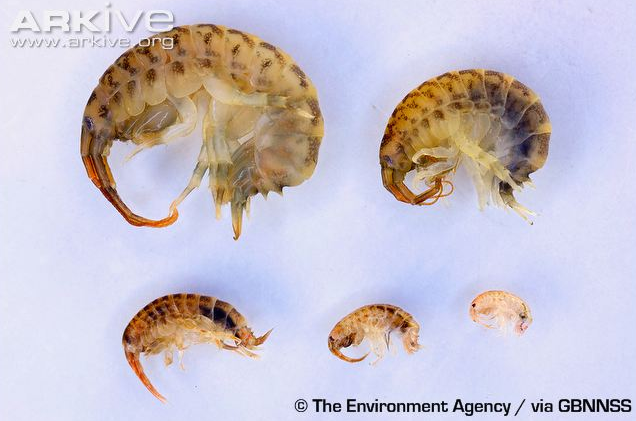
\includegraphics[width=8cm]{shrimpy1}}
\end{frame}

\begin{frame}{Killer Shrimp}
\centerline{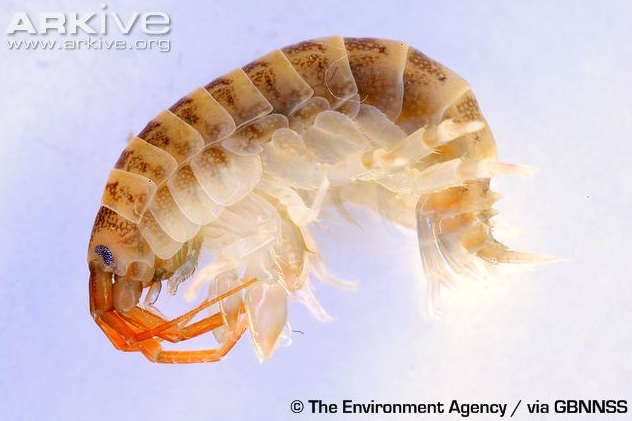
\includegraphics[width=8cm]{shrimpy2}}
\end{frame}

\begin{frame}{Killer Shrimp}
\centerline{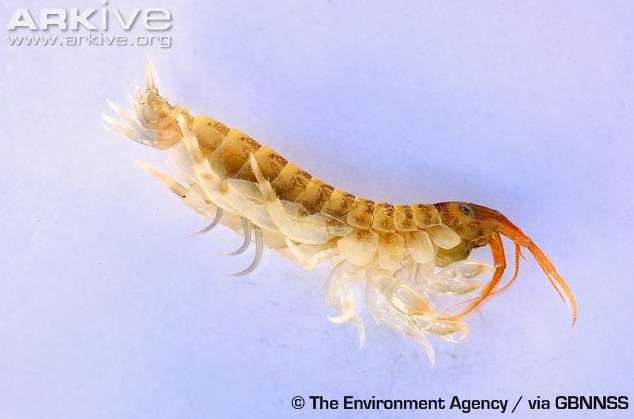
\includegraphics[width=8cm]{shrimpy3}}
\end{frame}

\begin{frame}
	\centerline{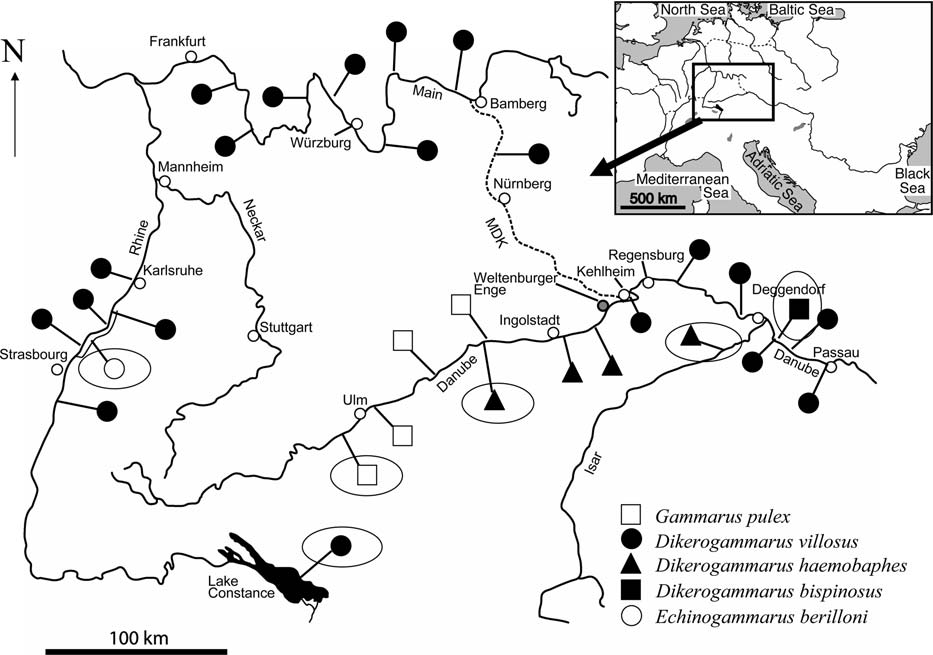
\includegraphics[width=10cm]{img/kinzlermap}}
	
	\center{(Kinzler, 2008)}
\end{frame}


\begin{frame}{Time Line}

  \vfill

  The time to prominence. 

  \vfill

  \begin{tabular}{l|l}
    Years      & Species \\ \hline
    $<$1976    & \textit{Gp} native\\
    1976-1994  & \textit{Dh} invades\\
    1992-1995  & \textit{Dv} invades, \textit{Dh} declines\\
    $>$1995    & All but \textit{Dv} coexist separate from \textit{Dv}
  \end{tabular}

  \vfill

\end{frame}

\begin{frame}
   \frametitle{Terminology}
	\begin{block}{Intraguild Predation}
		Mutual Predation\\
		Mutual Interference \\
	\end{block}
	\begin{block}{Intraspecific Predation}
		Cannibalism
	\end{block}
\end{frame}

\begin{frame}
   \frametitle{Kinzler, 2008 Study}
	\vfill
	
	Isolated pairs of specimens in a controlled environment
	\begin{itemize}
		\item One freshly moulted (prey) 
		\item One predator
		\item Total of 279 experiments
		\item Grouped by age, sex, and species
	\end{itemize}
	
\vfill
	Results\\
	\begin{itemize}
	\item Found \textit{Dv} to be clear strongest predator\\
\vspace{.5em}
	\item Found \textit{Dh} to have highest cannibalism rate
\end{itemize}

\vfill
\end{frame}

\begin{frame}
   \frametitle{Basic Goals}
\begin{center}
		{\Large{\textbf{Determine long term population trends!}}}\\


\vspace{2.5em}
		Does \textit{Dv} totally dominate in the end?\\
\vspace{.5em}
		Which species survive?\\
\vspace{.5em}

		Is there an equilibrium?

\end{center}

\end{frame}


%\begin{frame}
%  \frametitle{The Issues}
%
%  We gonna talk about the issues about talking about stuff.
%
%\end{frame}
%
%
%\begin{frame}
%  \frametitle{Random Stuff}
%
%  Random stuff is like totally out there.
%
%  \uncover<2->
%  {
%
%    It could just be totally surprising.
%
%  }
%
%  \uncover<3->
%  {
%
%    Unexpected even, you know what I mean?
%
%  }
%
%
%\end{frame}
%
%
%\subsection{Statistics}
%
%\begin{frame}{Statistics Do Not Lie}
%
%  You can totally trust the statistics.
%
%  \only<2>{
%
%    Well... usually
%    \begin{itemize}
%    \item We could make a type I error.
%    \item Or it could be a type II error.
%    \end{itemize}
%
%  }
%
%  \only<3-4>{
%
%    Then again maybe the hypothesis test does not even make sense.
%
%  }
%
%  \only<4->{
%
%    Then you are really hosed.
%
%  }
%
%\end{frame}




%\documentclass[12pt,letterpaper]{amsart}
%\setlength{\oddsidemargin}{.0in}
%\setlength{\evensidemargin}{.0in}
%\setlength{\textwidth}{6.5in}
%\setlength{\topmargin}{-.3in}
%\setlength{\headsep}{.20in}
%\setlength{\textheight}{9.in}
%\usepackage[leqno]{amsmath}
%\usepackage{amsfonts}
%\usepackage{amssymb}
%\usepackage{amsthm}
%\usepackage{amssymb}
%\usepackage[all]{xy}
%\usepackage{graphicx}



%Here are some user-defined notations
\newcommand{\RR}{\mathbf R}
\newcommand{\CC}{\mathbf C}
\newcommand{\ZZ}{\mathbf Z}
\newcommand{\ZZn}[1]{\ZZ/{#1}\ZZ}
\newcommand{\QQ}{\mathbf Q}
\newcommand{\rr}{\mathbb R}
\newcommand{\cc}{\mathbb C}
\newcommand{\zz}{\mathbb Z}
\newcommand{\zzn}[1]{\zz/{#1}\zz}
\newcommand{\qq}{\mathbb Q}
\newcommand{\calM}{\mathcal M}
\newcommand{\latex}{\LaTeX}
\newcommand{\tex}{\TeX}
\newcommand{\sm}{\setminus} 


%improving spacing in tables (space above and below characters in a row)
\newcommand{\tfix}{\rule{0pt}{2.6ex}}
\newcommand{\bfix}{\rule[-1.2ex]{0pt}{0pt}}



%Here are commands with variable inputs 
\newcommand{\intf}[1]{\int_a^b{#1}\,dx}
\newcommand{\intfb}[3]{\int_{#1}^{#2}{#3}\,dx}
\newcommand{\marginalfootnote}[1]{%
        \footnote{#1}
        \marginpar[\hfill{\sf\thefootnote}]{{\sf\thefootnote}}}
\newcommand{\edit}[1]{\marginalfootnote{#1}}


%Here are some user-defined operators
\newcommand{\Tr}{\operatorname {Tr}}
\newcommand{\GL}{\operatorname {GL}}
\newcommand{\SL}{\operatorname {SL}}
\newcommand{\Prob}{\operatorname {Prob}}
\newcommand{\re}{\operatorname {Re}}
\newcommand{\im}{\operatorname {Im}}


%These commands deal with theorem-like environments (i.e., italic)
%\theoremstyle{plain}
%\newtheorem{theorem}{Theorem}[section]
%\newtheorem{corollary}[theorem]{Corollary}
%\newtheorem{lemma}[theorem]{Lemma}
%\newtheorem{conjecture}[theorem]{Conjecture}

%These deal with definition-like environments (i.e., non-italic)
%\theoremstyle{definition}
%\newtheorem{definition}[theorem]{Definition}
%\newtheorem{example}[theorem]{Example}
%\newtheorem{remark}[theorem]{Remark}

%This numbers equations by section
\numberwithin{equation}{section}

%\begin{document}

\begin{frame}{Brownian Motion}
\begin{definition}(\textbf{Brownian Motion}) is a stochastic process that models random continuous motion. The stochastic process $B=\{B(t), t\geq 0\}$ is standard Brownian Motion if the following holds:
\begin{enumerate}
\item[(1)]
$B$ has independent increments.
\item[(2)]
For $0 \leq s < t,$ $$B(t)-B(s) \sim N(0,t-s),$$\\
meaning the increment $B(t)-B(s)$ is normally distributed with mean $0$ and variance equal to the length of the increment separating $s \ \text{and} \ t$
\item[(3)] With probability $1$, paths of $B$ are continuous; that is, $$P[B \in C[0, \infty)]=1.$$
\item[(4)] $B(0)=0$ 
\end{enumerate}
\end{definition}

The Brownian motion process, sometimes referred to as the Weiner process can be thought of as a continuous time approximation of a random walk where the size of the steps is called to become smaller and the rate at which steps are taken is speeded up. \\
\end{frame}


\begin{frame}
  %\frametitle{Without Noise}
  \movie[height=6.33cm,width=8.55cm,loop,poster]{Random Walk}{randomWalk.avi}

  \hyperlinkmovie[once]{randomWalk.avi}{Random Walk}
\end{frame}


\begin{frame}{Markov Process}
(\textbf{Markov Process}) is a stochastic process with the following properties: 
\begin{enumerate}
\item[(a.)] The number of possible outcomes or states if finite
\item[(b.)] The outcome at any stage depends only on the outcome of the previous stage.
\item[(c.)] The probabilities are constant over time.   
\end{enumerate}
\end{frame}

\begin{frame}
$$ \frac{x(\lambda t)}{\sqrt{\lambda}}$$ is a Brownian motion. 

\begin{align*}
 & \frac{x(\lambda t)}{\sqrt{\lambda}}-\frac{x(\lambda s)}{\sqrt{\lambda}}\\
 & P \left(a \leq \frac{x(\lambda t)}{\sqrt{\lambda}}-\frac{x(\lambda s)}{\sqrt{\lambda}} \leq b \right)=P \left(a \sqrt{\lambda} \leq x(\lambda t) - x (\lambda s) \leq b \sqrt{\lambda} \right)\\
 & \displaystyle \frac{1}{\sqrt{2 \pi (\lambda t -\lambda s)}} \int_{a \sqrt{\lambda}}^{b \sqrt{\lambda}} e^{\frac{-x^2}{2}(\lambda t- \lambda s)} dx\\
  & u=\frac{x}{\sqrt{\lambda}}\\
  & du=\frac{1}{\sqrt{\lambda}}\\
  & =\frac{1}{\sqrt{2 \pi \lambda(t-s)}} \int_{a}^{b} e^{\frac{-u^2}{t-s}} \cdot \sqrt{\lambda}du\\
  & = \frac{1}{\sqrt{2 \pi (t-s)}} \int_{a}^{b} e^{\frac{-u^2}{t-s}}du
 \end{align*}
 

Brownian motion because has a $\mu=0 \ \text{and} \ \sigma^2=t-s$

\end{frame}

\begin{frame}{Riemann-Stieltjes}
(\textbf{Riemann-Stieltjes Integral}): 
$$\displaystyle \int_{a}^{b} f(g)dg= \underset{n \to \infty}{\lim} \sum_{i=1}^{N} f(g(t_i)) \cdot (g(t_{i+1}))- g(t_i))$$\\

The main motivation for the Riemann-Stieltjes Integral comes from the concept of Cumulative Distribution Function (CDF) of a random variable. 
\end{frame}

\begin{frame}{Weiner Integral}
\textbf{Weiner Integral} $$\int_{a}^{b} f(t)dW(t)$$
$$1[t_{i+1}, t_i] (t)= \begin{cases} 1 & \text{if} \ t_{i+1} \leq t < t_i \\
0 & \text{otherwise} \end{cases}$$
\end{frame}


%\textbf{Multivariate Taylor Expansion:} $$F(t)-F(s)=F^{\prime}(s)(t-s)+\frac{1}{2}F^{''} (s)(t-s)^2 + \frac{1}{3!}F^{'''}(t-s)^3+ \text{H.O.T}$$

\begin{frame}{It\^o's Formula}
\textbf{It\^{o}'s Formula} $$\displaystyle F(t, B(t))-F(a,B(a))=
 \int_{a}^{t} \frac{\partial F}{\partial s} + \frac{1}{2} \frac{\partial^2 F}{\partial B^2}ds+
 \int_a^t \frac{\partial F}{\partial B} dB$$

Let $F=tB^2$ 
\begin{align*}
\displaystyle
&\frac{dF}{dt}= B^2\\
&\frac{dF}{dB}=2t+B\\ 
&\frac{d^2 F}{dB^2}=2t
\end{align*}
\begin{align*}
tB^2(t)-aB^2(a) &=\int_{a}^{t}B^s ds+ \int_{a}^{t}2sBdB+\int_a^t \frac{1}{2}2sds\\
 &=\int_a^b B^2+sds+\int_a^t 2sBdB\\
 &\text{OR}\\
tB^2(t)-aB^2(a) &= \int_a^t B^s ds+ \int_a^t 2sBdBt+ \frac{1}{2} t^2- \frac{1}{2}a^2
\end{align*}
\end{frame}

\begin{frame}{Example of It\^o's Formula}
Use It\^o's formula to find an integral expression for the following integraL:
$$f(B)=B^4$$
\begin{align*}
f(x)&=B^4\\
f'(x)&=4B^3\\
f''(x)&=12B^2\\
d(B^4)&= 4B^3(t)dB+\frac{1}{2}(12B(t)^2)dt\\
	&=4B^3(t)dB+6B^2(t)dt\\
B^4(t)&= 4 \int_0^t B^3 dB+ 6 \int_0^t B^2 ds\\
E\left[\int_0^t B_s^2 ds\right] &= \frac{1}{6}E \left[B_t^4-4 \int_0^tB_s^3 dBs \right]\\
 &=\frac{1}{6}  \left[E \left[B_t^4\right]-4E\left[\int_0^t B_s^3 dBs \right] \right]\\
 &=\frac{1}{6}(3t^2)
\end{align*}
\end{frame}

\begin{frame}{Nondimensionalization}
\textbf{Nondimensionalization}: method to reduce parameters. 

\begin{enumerate}
\item
List all the variables and parameters along with their dimensions.
\item
For each variable, say $x$, form a product (or quotient) $p$ of parameters that has the same dimensions as $x$, and define a new variable $y=\frac{x}{p}.$ $y$ is a "dimensionless" variable. It's numberical  value is the same no matter what system of units is used.
\item Rewrite the differential equation in terms of the new variables.
\item 
In the new differential equation, group the parameters into nondimensional combinations, and define a new set of nondimensional parameters expressed as the nondimensional combinations of the original parameters. 
\end{enumerate}
\end{frame}

\begin{frame}{Killer Shrimp}
\centerline{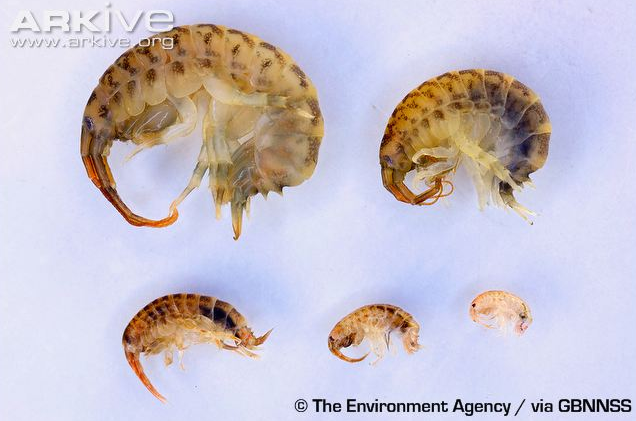
\includegraphics[width=8cm]{shrimpy1}}
\end{frame}

\begin{frame}{Killer Shrimp}
\centerline{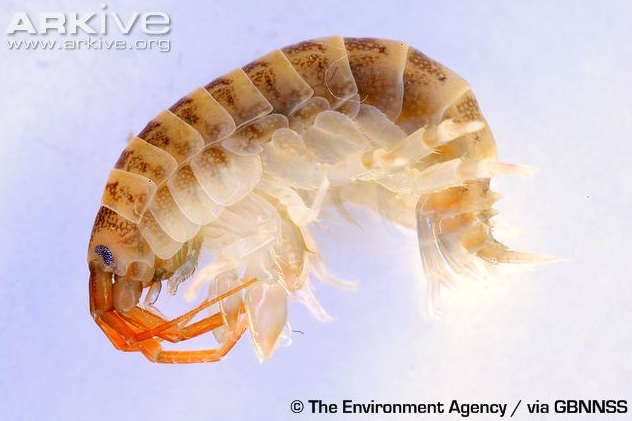
\includegraphics[width=8cm]{shrimpy2}}
\end{frame}

\begin{frame}{Killer Shrimp}
\centerline{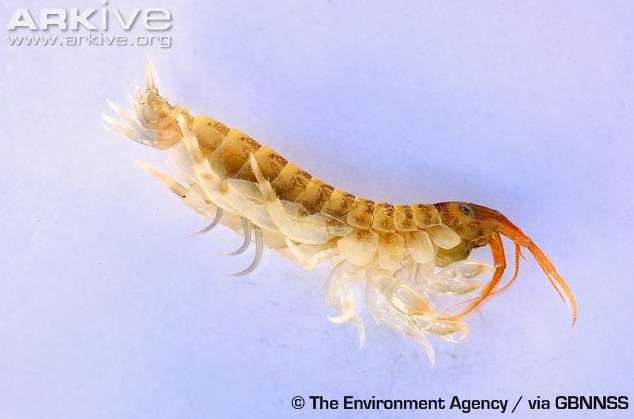
\includegraphics[width=8cm]{shrimpy3}}
\end{frame}

%\end{document}





\numberwithin{equation}{section}

\section{Stochastic Calculus}
\begin{frame}
  \frametitle{Outline}
  \tableofcontents[ currentsection]
\end{frame}



\subsection{Stochastic Integration}

\begin{frame}
  \frametitle{Overview}

  The governing Equations:
  \begin{eqnarray*}
    \dot{a} & = & L_1a + N_1(a,g), \\
    \dot{g} & = & L_2g + N_2(a,g).
  \end{eqnarray*}


\end{frame}

\begin{frame}
	\frametitle{Calculating Stochastic Integrals}
		As an example consider the integral 
			$$Z_t=\int_0^t B(s) dB(s)$$
			
		This integral can be calculated as
			$$\displaystyle \int_0^t B(s)dB(s)=\frac{1}{2}(B^2(t)-B^2(0))-\frac{1}{2}$$
			
			% % can go over this calculation during presentation using Taylor Expansion
			
\end{frame}





\begin{frame}
  \frametitle{The ``Usual Scaling''}
  \begin{eqnarray*}
    x & \rightarrow & \bar{X} \xi, \\
    t & \rightarrow & \bar{T} s.
  \end{eqnarray*}

\end{frame}

%\begin{frame}
  %\frametitle{The Finite Difference Approximation}

  %\begin{itemize}
  %\item<4-> Usual stability issues.
  %\item<3-> Usual ease of use.
  %\item<2-> Usual wave speed problem.
  %\item<1-2> Usual centered difference scheme.
  %\end{itemize}
  %\uncover<3->{Don't that beat all?}

%\end{frame}


\subsection{Stochastic Differential Equations}

%\begin{frame}
 % \frametitle{Comparison}

  %\begin{columns}[t]
   % \column{.5\textwidth}
    %\centerline{\includegraphics[height=5.0cm]{gainComp-001}}
    %This is what the left looks like

    %\column{.5\textwidth}
    %\centerline{\includegraphics[height=5.0cm]{energyComp-001}}
    %This is what the right looks like

  %\end{columns}

%\end{frame}


%\subsection{Random Thoughts}
%\begin{frame}
 % \frametitle{Random Thoughts}
  %But what about Barney and PBS?

  %\begin{columns}[t]
    
   % \column{.5\textwidth}
    %\begin{block}{Barney?}
     % Is it okay to trust your kids with Barney?
    %\end{block}
    %\pause
  
    %\column{.5\textwidth}
    %\begin{block}{No, not Barney!}
     % Probably not.
    %\end{block}

  %\end{columns}


%\end{frame}



\numberwithin{equation}{section}

\section{Modeling}
\begin{frame}
  \frametitle{Outline}
  \tableofcontents[ currentsection ]
\end{frame}

\begin{frame}{Shrimp Model}
  \begin{align*}
    \frac{dx}{dt} & = rx^2 \left(1-\frac{x}{K}\right) - \alpha xy - \frac{x^2 \gamma_\circ}{x+D}, \\
    \frac{dy}{dt} & = \rho y^2 \left(1-\frac{y}{L}\right) - \beta xy -\frac{y^2 \delta_\circ}{y+R}.
  \end{align*}
\end{frame}

\numberwithin{equation}{section}

\subsection{Nondimensionalization}
%\begin{frame}
  %\frametitle{Outline}
  %\tableofcontents[ currentsection ]
%\end{frame}

\begin{frame}
\frametitle{Nondimensionalization}

  The nondimensionalized system is:

	\begin{align*}
		\frac{dx}{dt} &= x^2 (1-x) - \alpha xy - \frac{\gamma_\circ x^2}{x+D}, \\
    \frac{dy}{dt} &= \rho y^2 (1-y) - \beta xy -\frac{\delta_\circ y^2}{y+R}
	\end{align*}
\end{frame}

\begin{frame}
  %\movie[height=6.33cm,width=8.55cm,loop,poster]{Milstein Process}{Milstein.mp4}
\end{frame}



\begin{frame}{Phase Plane}

  \vfill
	
  \begin{columns}
    \only<1> {
      \column{.65\textwidth}
      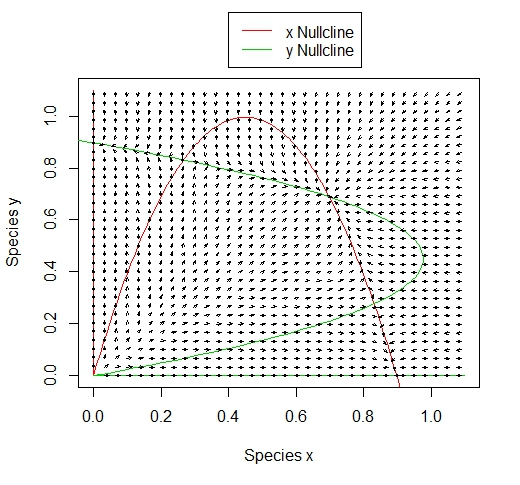
\includegraphics[height=7cm]{img/RplotMain}
      \column{.35\textwidth}
      $\alpha = .2, \beta = .2,
      \gamma = .8, \delta = .4, \rho = 1, R = 3$ and $D = 7$ 

      \begin{itemize}
      \item Six fixed points.
      \item Three are unstable.
      \end{itemize}
    }

    \only<2> {
      \column{.65\textwidth}
      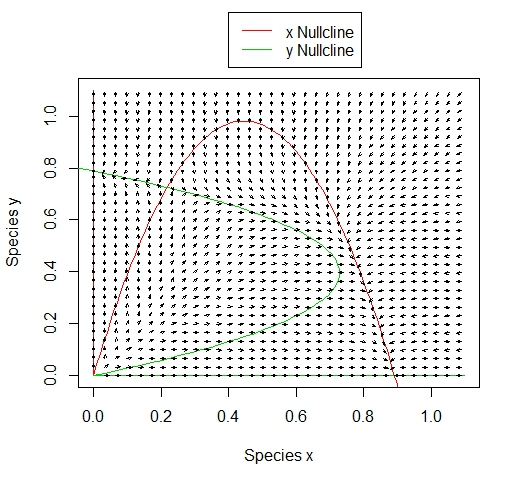
\includegraphics[height=7cm]{img/Rplot1} 
      \column{.35\textwidth}
      $\gamma = .85$ and $\delta = .8$ 
      \begin{itemize}
      \item Four fixed points.
      \item Two are unstable.
      \end{itemize}
    }

    \only<3> {
      \column{.65\textwidth}
      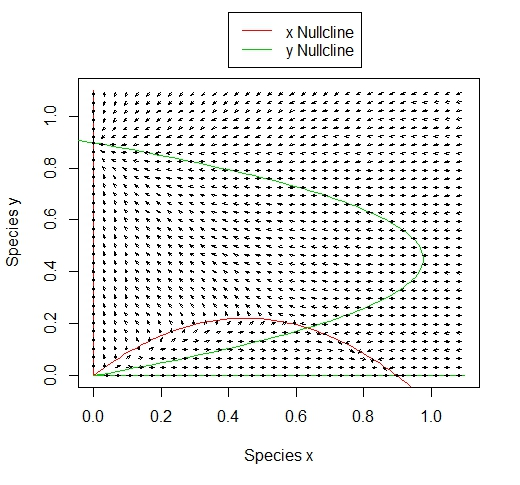
\includegraphics[height=7cm]{img/Rplot2} 
      \column{.35\textwidth}
      $\alpha = .9, \beta = .2, \gamma = .8$ and $\delta = .4$
      \begin{itemize}
      \item Four fixed points.
      \item Two are unstable.
      \end{itemize}
    }

    \only<4> {
      \column{.65\textwidth}
      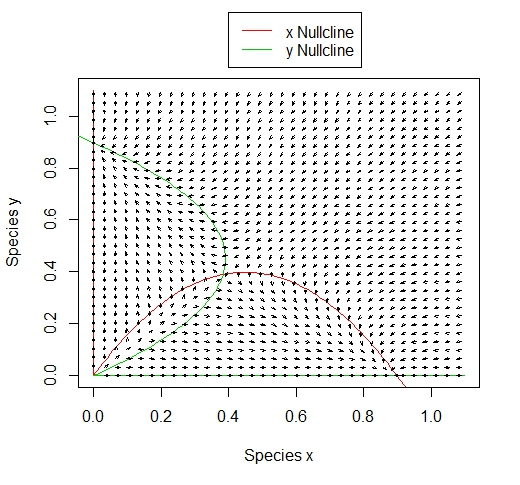
\includegraphics[height=7cm]{img/Rplot3} 
      \column{.35\textwidth}
      $\alpha = .5, \beta = .5, \gamma = .8$ and $\delta = .4$ 
      \begin{itemize}
      \item Four fixed points.
      \item Two are unstable.
      \end{itemize}
    }

    \only<5> {
      \column{.65\textwidth}
      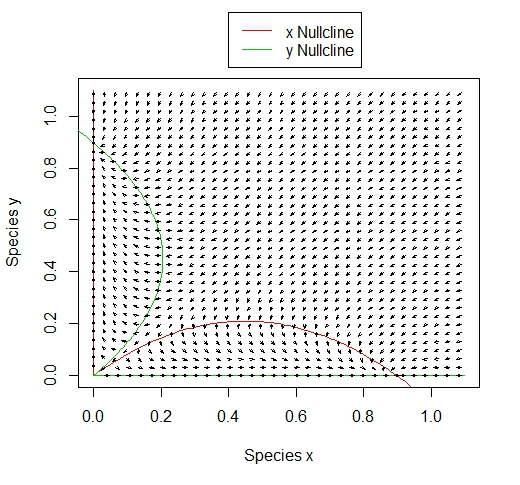
\includegraphics[height=7cm]{img/Rplot4} 
      \column{.35\textwidth}
      $\alpha = .95, \beta = .95, \gamma = .8$ and $\delta = .4$ 
      \begin{itemize}
      \item Three fixed points.
      \item One is unstable.
      \end{itemize}
    }

  \end{columns}
\end{frame}




\begin{frame}{Noise}

  Additive noise...
  \begin{align*}
    \frac{dx}{dt} &= x^2 (1-x) - \alpha xy - \frac{\gamma_\circ x^2}{x+D} + \upsilon \frac{dW}{dt}, \\
    \frac{dy}{dt} &= \rho y^2 (1-y) - \beta xy -\frac{\delta_\circ y^2}{y+R}+ \kappa \frac{dB}{dt}.
  \end{align*}

  Proportional noise...
  \begin{align*}
    \frac{dx}{dt} &= x^2 (1-x) - \alpha xy - \frac{\gamma_\circ x^2}{x+D} + \upsilon x \frac{dW}{dt}, \\
    \frac{dy}{dt} &= \rho y^2 (1-y) - \beta xy -\frac{\delta_\circ y^2}{y+R}+ \kappa y \frac{dB}{dt}.
  \end{align*}

\end{frame}


%
%
%\begin{frame}
%\frametitle{Heun's Method}
%\begin{itemize}
%\item Heun's method is a numerical procedure for approximating ordinary differential equations with a given initial value.
%\item First you calculate the intermediate value $\tilde{y}_{i+1}$ and then the final approximation $y_{i+1}$ at the next generation point.
%\end{itemize}
%
%\begin{align*}
%	\tilde{y}_{i+1} &= y_i + \Delta t \ f(t_i, y_i) \\
%	y_{i+1} &= y_i + \frac{\Delta t}{2} \left[f(y_i,t_i) + f(\tilde{y}_{i+1}, t_{i+1})\right]
%\end{align*}
%\end{frame}
%
%
%\begin{frame}
%   \frametitle{Heun's Method vs. Euler's Method - Simulation}
%For the DE $y'=r y$ on $[0,T]$,\\
%\vspace{1em}
%	%\hspace{1.5em} Heun's:$\hspace{1em} \tilde{y}_{i+1} = y_i + \Delta t \ f(t_i, y_i)$ \\
%		\hspace{1.5em} Heun's:$ \hspace{1em} y_{i+1} = y_i + \frac{\Delta t}{2} \left[f(y_i,t_i) + f(\tilde{y}_{i+1}, t_{i+1})\right]$ \vspace{1em} \\
%	\hspace{1.5em} Euler's:$\hspace{1em}\tilde{y}_{i+1} = y_i + \Delta t \ f(y_i, t_i)$ \\
%\begin{columns}[t]
%    \column{.5\textwidth} 
%    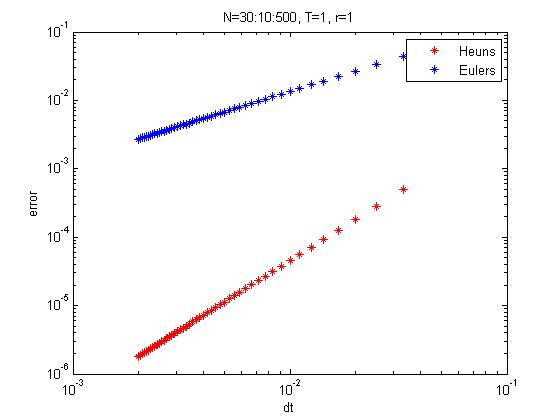
\includegraphics[width=6cm]{img/Heun500}
%    \column{.5\textwidth}
%    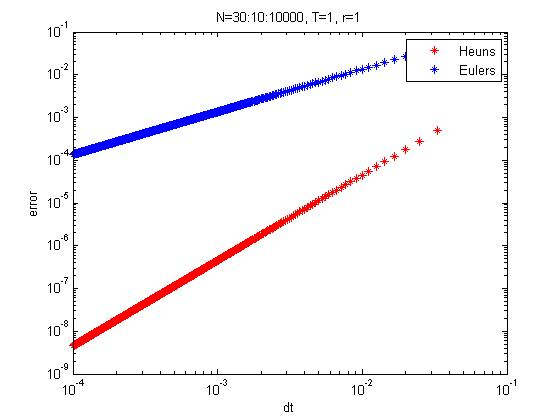
\includegraphics[width=6cm]{img/Heun10000}
%  \end{columns}
%
%\end{frame}




\end{document}

